\section{Sistemas de enclavamiento}
	\label{sec:interlockingTheory}
	
	Tal cómo fue definido en la Sección \ref{sec:topologias}, un sistema de enclavamientos debe gestionar las rutas ferroviarias, utilizando el señalamiento para otorgarle al conductor ferroviario autoridad o no sobre ciertas secciones de la red ferroviaria. Las decisiones se toman en base al estado actual de los elementos ferroviarios que componen la red y considerando qué estado garantiza una mayor seguridad, al impedir descarrilamientos y colisiones.
	
	Existen diversas funcionalidades que complementan al sistema de enclavamientos. Algunas centradas en incrementar la seguridad general del sistema y otras en flexibilizar la logística de la asignación de rutas. En esta sección se describirán seis de las funcionalidades principales del sistema de enclavamientos implementadas por el ACG.
	
	\subsection{Bloqueo de máquina de cambios por ocupación}

	\label{sec:function_1}

	Evitar el descarrilamiento de las formaciones es una de las funciones del sistema de enclavamientos. Esto puede ocurrir principalmente en dos situaciones: formaciones circulando a alta velocidad en las curvas o conmutaciones en la máquina de cambios mientras una formación circula sobre el cambio de vías. Para evitar este último escenario, el sistema de enclavamientos implementa un bloqueo de la máquina de cambios por ocupación, tal como se ilustra en la Figura \ref{fig:ACG_ocupacion}.

    \begin{figure}[!h]
        \centering
        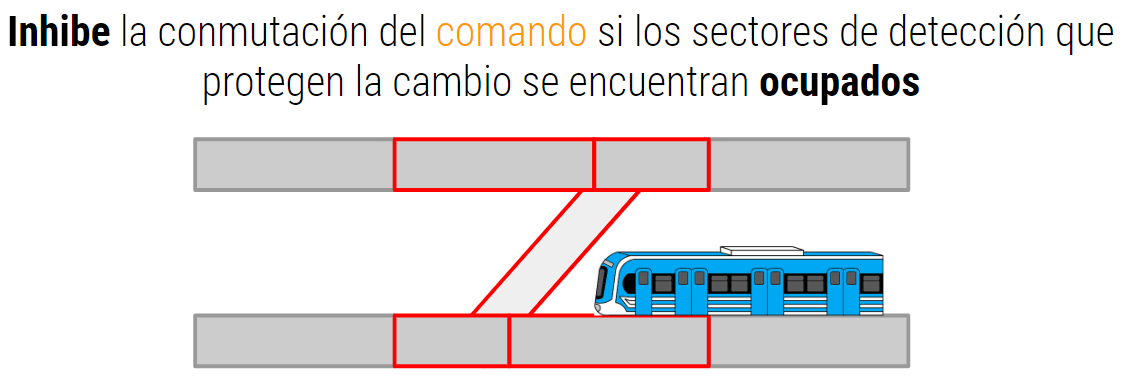
\includegraphics[width=1\textwidth]{Figuras/ocupacion}
        \centering\caption{Bloqueo de máquina de cambios por ocupación de secciones adyacentes.}
        \label{fig:ACG_ocupacion}
    \end{figure}

	La funcionalidad implementada radica en inhibir la conmutación de la máquina de cambios si alguna de las secciones de vías próximas al cambio de vías se encuentra ocupada. De esta manera, se garantiza que la posición del cambio de vías se mantendrá al detectar una formación aproximándose y no se permitirá su conmutación hasta que la formación se encuentre completamente alejada una distancia de seguridad. 
	\subsection{Requerimiento de rutas y bloqueo de cambios en ruta}

\lipsum[1]
    \begin{figure}[!h]
        \centering
        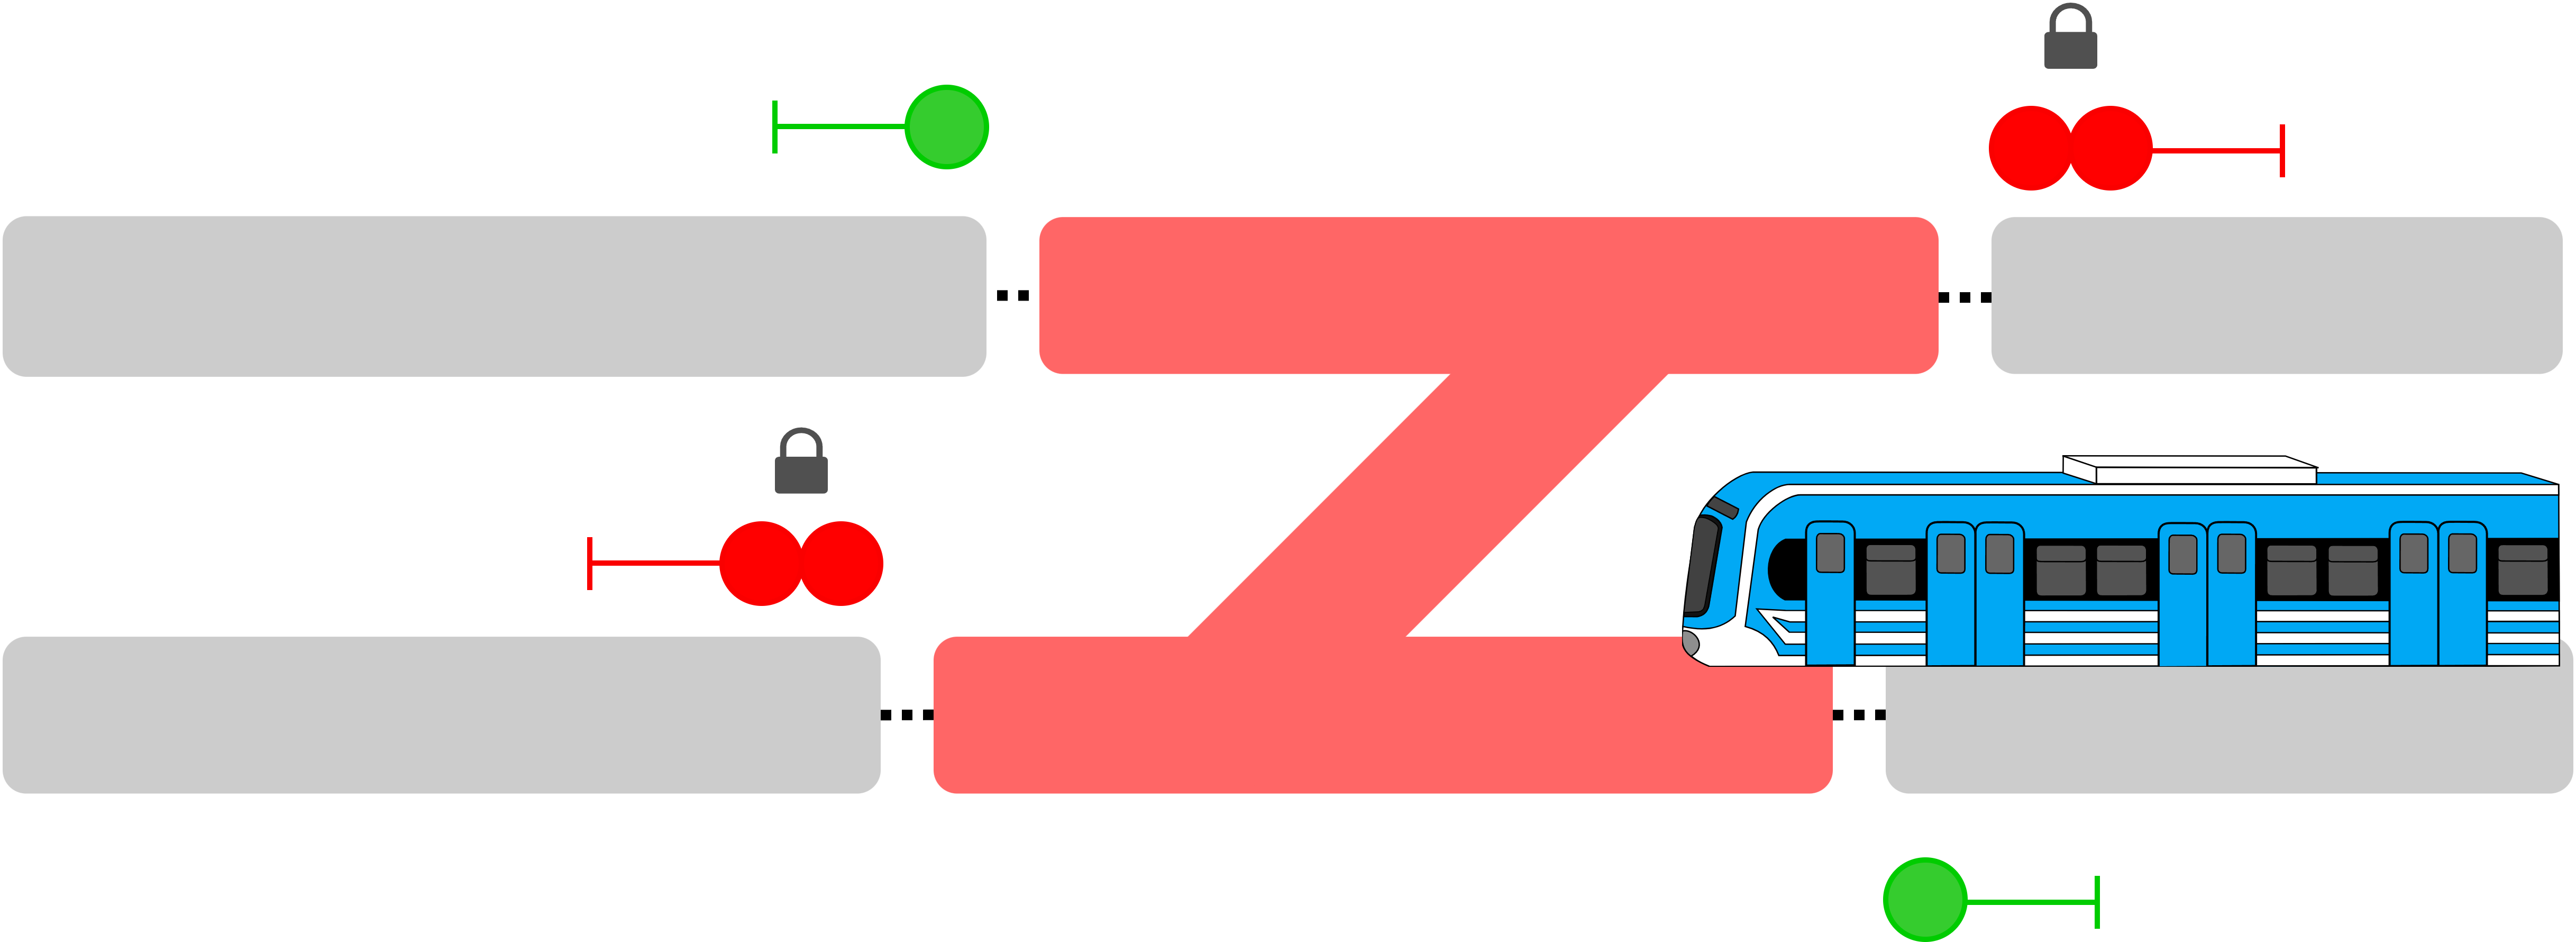
\includegraphics[width=1\textwidth]{Figuras/bloqueo_rutas}
        \centering\caption{XXXXX.}
        \label{fig:ocupacion_1}
    \end{figure}
\lipsum[1]
	\subsection{Protección por aproximación en cancelación de ruta}

	\label{sec:function_3}
	
	La distancia de frenado es un aspecto esencial a considerar cuando una ruta en curso es cancelada. La ruta en cuestión debe seguir protegida durante un tiempo de seguridad.
	
	La Figura \ref{fig:ACG_aproximacion_1} introduce el caso de una formación que tenía una ruta aprobada (aspecto verde) que comenzaba en la sección violeta y abarcaba toda la sección naranja. Por seguridad, ambos cambios de vías fueron bloqueados y sus respectivas señales contrarias fueron forzadas a aspecto rojo y bloqueadas.

    \begin{figure}[!h]
        \centering
        
\includegraphics[width=1\textwidth]{Figuras/aproximacion_1}
        \centering\caption{Formación aproximándose al inicio de la ruta.}
        \label{fig:ACG_aproximacion_1}
    \end{figure}
    
    Mientras la formación se encuentra en movimiento, el operador solicitó la cancelación de la ruta, cambiando el aspecto de la señal a rojo, tal como se visualiza en la Figura \ref{fig:ACG_aproximacion_2}. La formación quizás no tenga el tiempo ni la distancia suficiente para detenerse antes de la señal, por lo que se presentan dos escenarios. 
    
    \begin{figure}[!h]
        \centering
        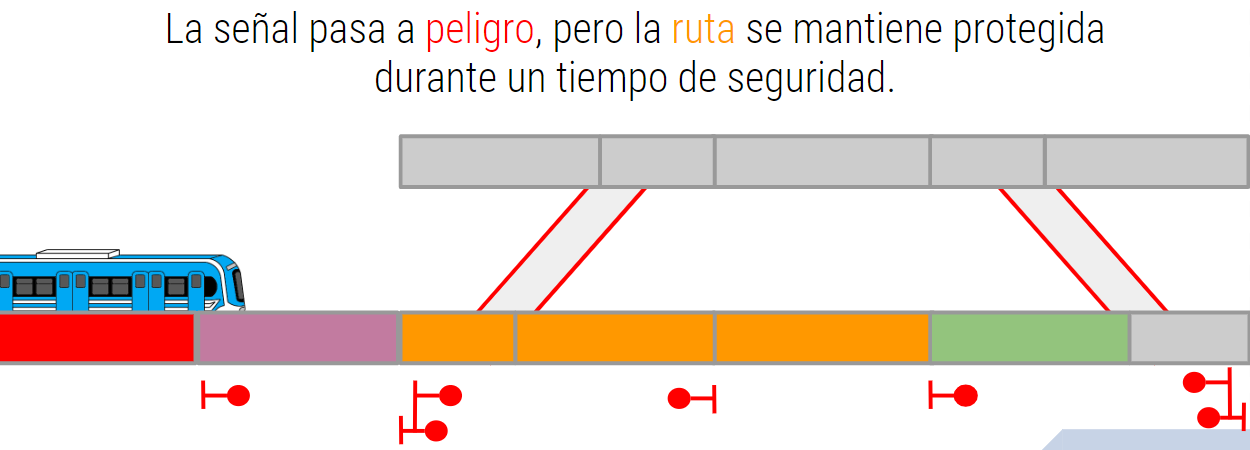
\includegraphics[width=1\textwidth]{Figuras/aproximacion_2}
        \centering\caption{La ruta es cancelada mietnras la formación se aproxima.}
        \label{fig:ACG_aproximacion_2}
    \end{figure}
    
    El primer escenario es el mas favorable: la formación se detiene previo a la señal de peligro y se inicia un contador. Al cumplirse el tiempo de seguridad, las secciones asociadas a la ruta cancelada son liberadas. Lo mismo sucede con los cambios de vías y las señales conflictivas. Este tiempo otorgado permite comprobar que la formación efectivamente se detuvo antes de proceder con la liberación de los elementos ferroviarios para que puedan ser utilizados por otra ruta.
    
    \begin{figure}[!h]
        \centering
        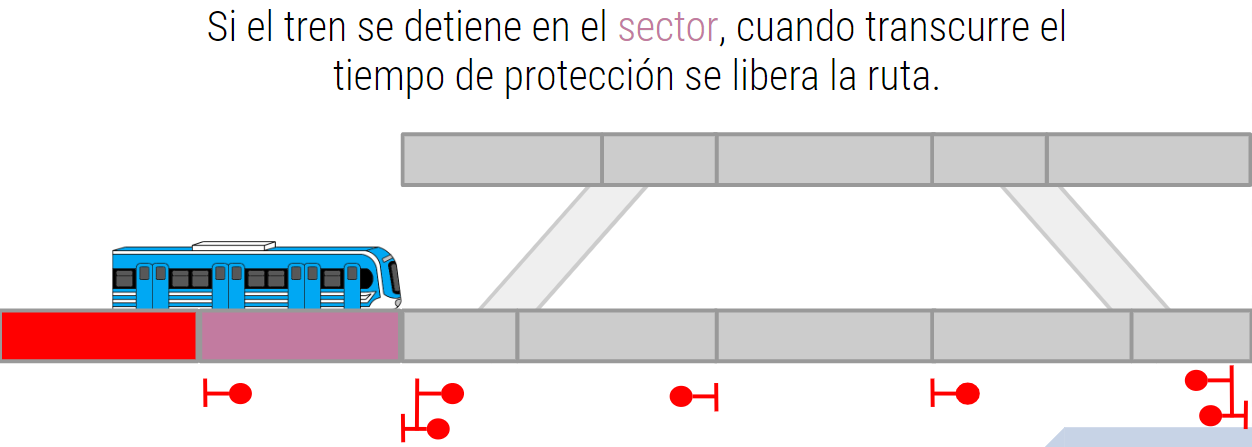
\includegraphics[width=1\textwidth]{Figuras/aproximacion_3}
        \centering\caption{La formación se detiene exitosamente previo a la señal de peligro.}
        \label{fig:ACG_aproximacion_3}
    \end{figure}
    
	En el segundo escenario, la formación no logra detenerse previo a la señal de peligro, tal como se ilustra en la Figura \ref{fig:ACG_aproximacion_4}. Entonces, el sistema de enclavamiento no solamente no libera las secciones pertenecientes a la ruta cancelada, sino que también bloquea las próximas secciones, al no poder estimar cual será la distancia final de frenado de la formación.

    \begin{figure}[!h]
        \centering
        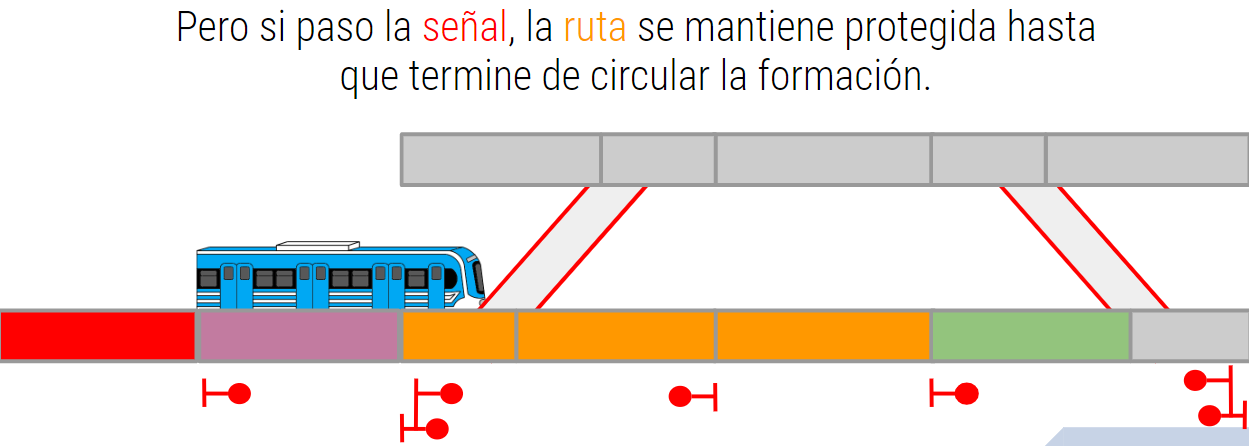
\includegraphics[width=1\textwidth]{Figuras/aproximacion_4}
        \centering\caption{La formación no se detiene previo a la señal de peligro.}
        \label{fig:ACG_aproximacion_4}
    \end{figure}
    
	Las secciones y elementos ferroviarios próximos se mantienen protegidos y enclavados hasta que la ruta se concluya, aún habiendo sido cancelada. Al finalizar la ruta, el sistema de enclavamiento liberará las secciones y elementos ferroviarios próximos al comprobarse que la formación se detuvo previo a la señal de finalización de la ruta.
	
	\subsection{Protección por solape}

	Si una formación no detiene su marcha antes de una señal de peligro, el sistema de enclavamiento debe bloquear las secciones pertenecientes a esa ruta y la próxima, junto con la infraestructura asociado. La Figura \ref{fig:ACG_solape_1} ilustra este suceso, donde una formación ingresa a la sección violeta pasando una señal a peligro, sin tener la autorización requerida. A diferencia de la protección por aproximación, donde una formación no logra detenerse antes de ingresar a una ruta cancelada con poca anticipación, la protección por solape se ocupa de proteger la infraestructura en el caso de que la formación ingrese a una ruta que jamás fue habilitada.

    \begin{figure}[!h]
        \centering
        
\includegraphics[width=1\textwidth]{Figuras/solape}
        \centering\caption{Formación ignora señal a peligro y se activa la protección por solape.}
        \label{fig:ACG_solape_1}
    \end{figure}
    
    Automáticamente, las secciones de la próxima ruta (coloreadas en naranja) son bloqueadas, a la vez que los cambios de vías cercanos y todas las señales tanto consecutivas como contrarias o convergentes. El bloqueo se removerá una vez que la formación se detenga en la próxima señal a peligro, luego de un tiempo de seguridad.
	\subsection{Doble recubrimiento}
	\label{sec:function_5}
	
	Para evitar que una formación colisione con otra formación que se encuentre detenida más adelante en la misma vía o circulando a menor velocidad, el sistema de enclavamiento deberá controlar las señales entre ambas para regular la velocidad y distancia entre ellas. Tal como se explicó en la Sección \ref{sec:signals}, las señales pueden presentar diferentes aspectos. Cada aspecto determinará un rango de velocidad permitido, siendo rojo el mas restrictivo. La Figura \ref{fig:ACG_recrubrimiento_1} ilustra el comportamiento del señalamiento cuando dos formaciones circulan en el mismo sentido, separadas por una distancia de seguridad.
	
	\begin{figure}[!h]
		\centering
		\includegraphics[width=1\textwidth]{Figuras/recubrimiento}
		\centering\caption{Protección por doble recubrimiento.}
		\label{fig:ACG_recrubrimiento_1}
	\end{figure}
	
	La formación que circula por detrás (formación A en la Figura \ref{fig:ACG_recrubrimiento_1}) se encuentra frente a una señal de aspecto verde, por lo
	que puede continuar su marcha sin restricciones, siempre y cuando su velocidad sea menor a la velocidad máxima permitida en la red ferroviaria. Si la formación A reduce la distancia a la formación B, pasará a estar regida por una señal de aspecto amarillo. Si esto sucediera, la formación A deberá disminuir su velocidad para volver a situarse dentro de una sección verde. Lo mismo ocurriría si la formación A alcanzara una señal de aspecto doble amarillo, indicada mediante la señal naranja en la Figura 3.8. En este caso dado que la distancia entre formaciones es aún menor, deberá reducirse aún más la velocidad.
	
	Si la formación A continúa con una mayor velocidad que la formación B, la distancia entre ambas se reducirá y el señalamiento que la formación A tiene en su camino le impondrá velocidades más y más reducidas, hasta que la distancia entre ambas formaciones se incremente a un valor seguro.
		
	Debido al bloqueo por ocupación, todas las secciones ocupadas por una formación presentan una señal a peligro (roja). Inmediatamente detrás de cada formación se genera una secuencia de señales denominada doble recubrimiento. Si la formación avanza y cambia de sección, las señales de protección cambiarán su aspecto acorde al movimiento de la formación, de forma tal que siempre la sección donde está la formación tenga su señal de protección en rojo, la sección anterior en amarillo, la sección anterior en doble amarillo y la sección anterior en verde. Si no hay ninguna formación en la sección anterior a la que tiene su señal en verde, entonces esa sección también tendrá su señal en verde, lo mismo que todas las secciones anteriores, hasta que haya una formación que ocupe una sección, en cuyo caso esa sección estará en rojo y la secuencia de doble recubrimiento se repetirá también detrás de esa formación.
	 
	La cantidad de señales y la secuencia de aspectos variará según el operador de la red, las normas locales o nacionales. Algunos países como el Reino Unido \cite{UK} utilizan la secuencia rojo-doble amarillo-amarillo-verde (Figura \ref{fig:uk_signalling}) y esta es la secuencia de aspectos que implementa el ACG en este trabajo, aunque cabe aclarar que el ACG puede modificarse para implementar otras secuencias. 
	
	\begin{figure}[!h]
		\centering
		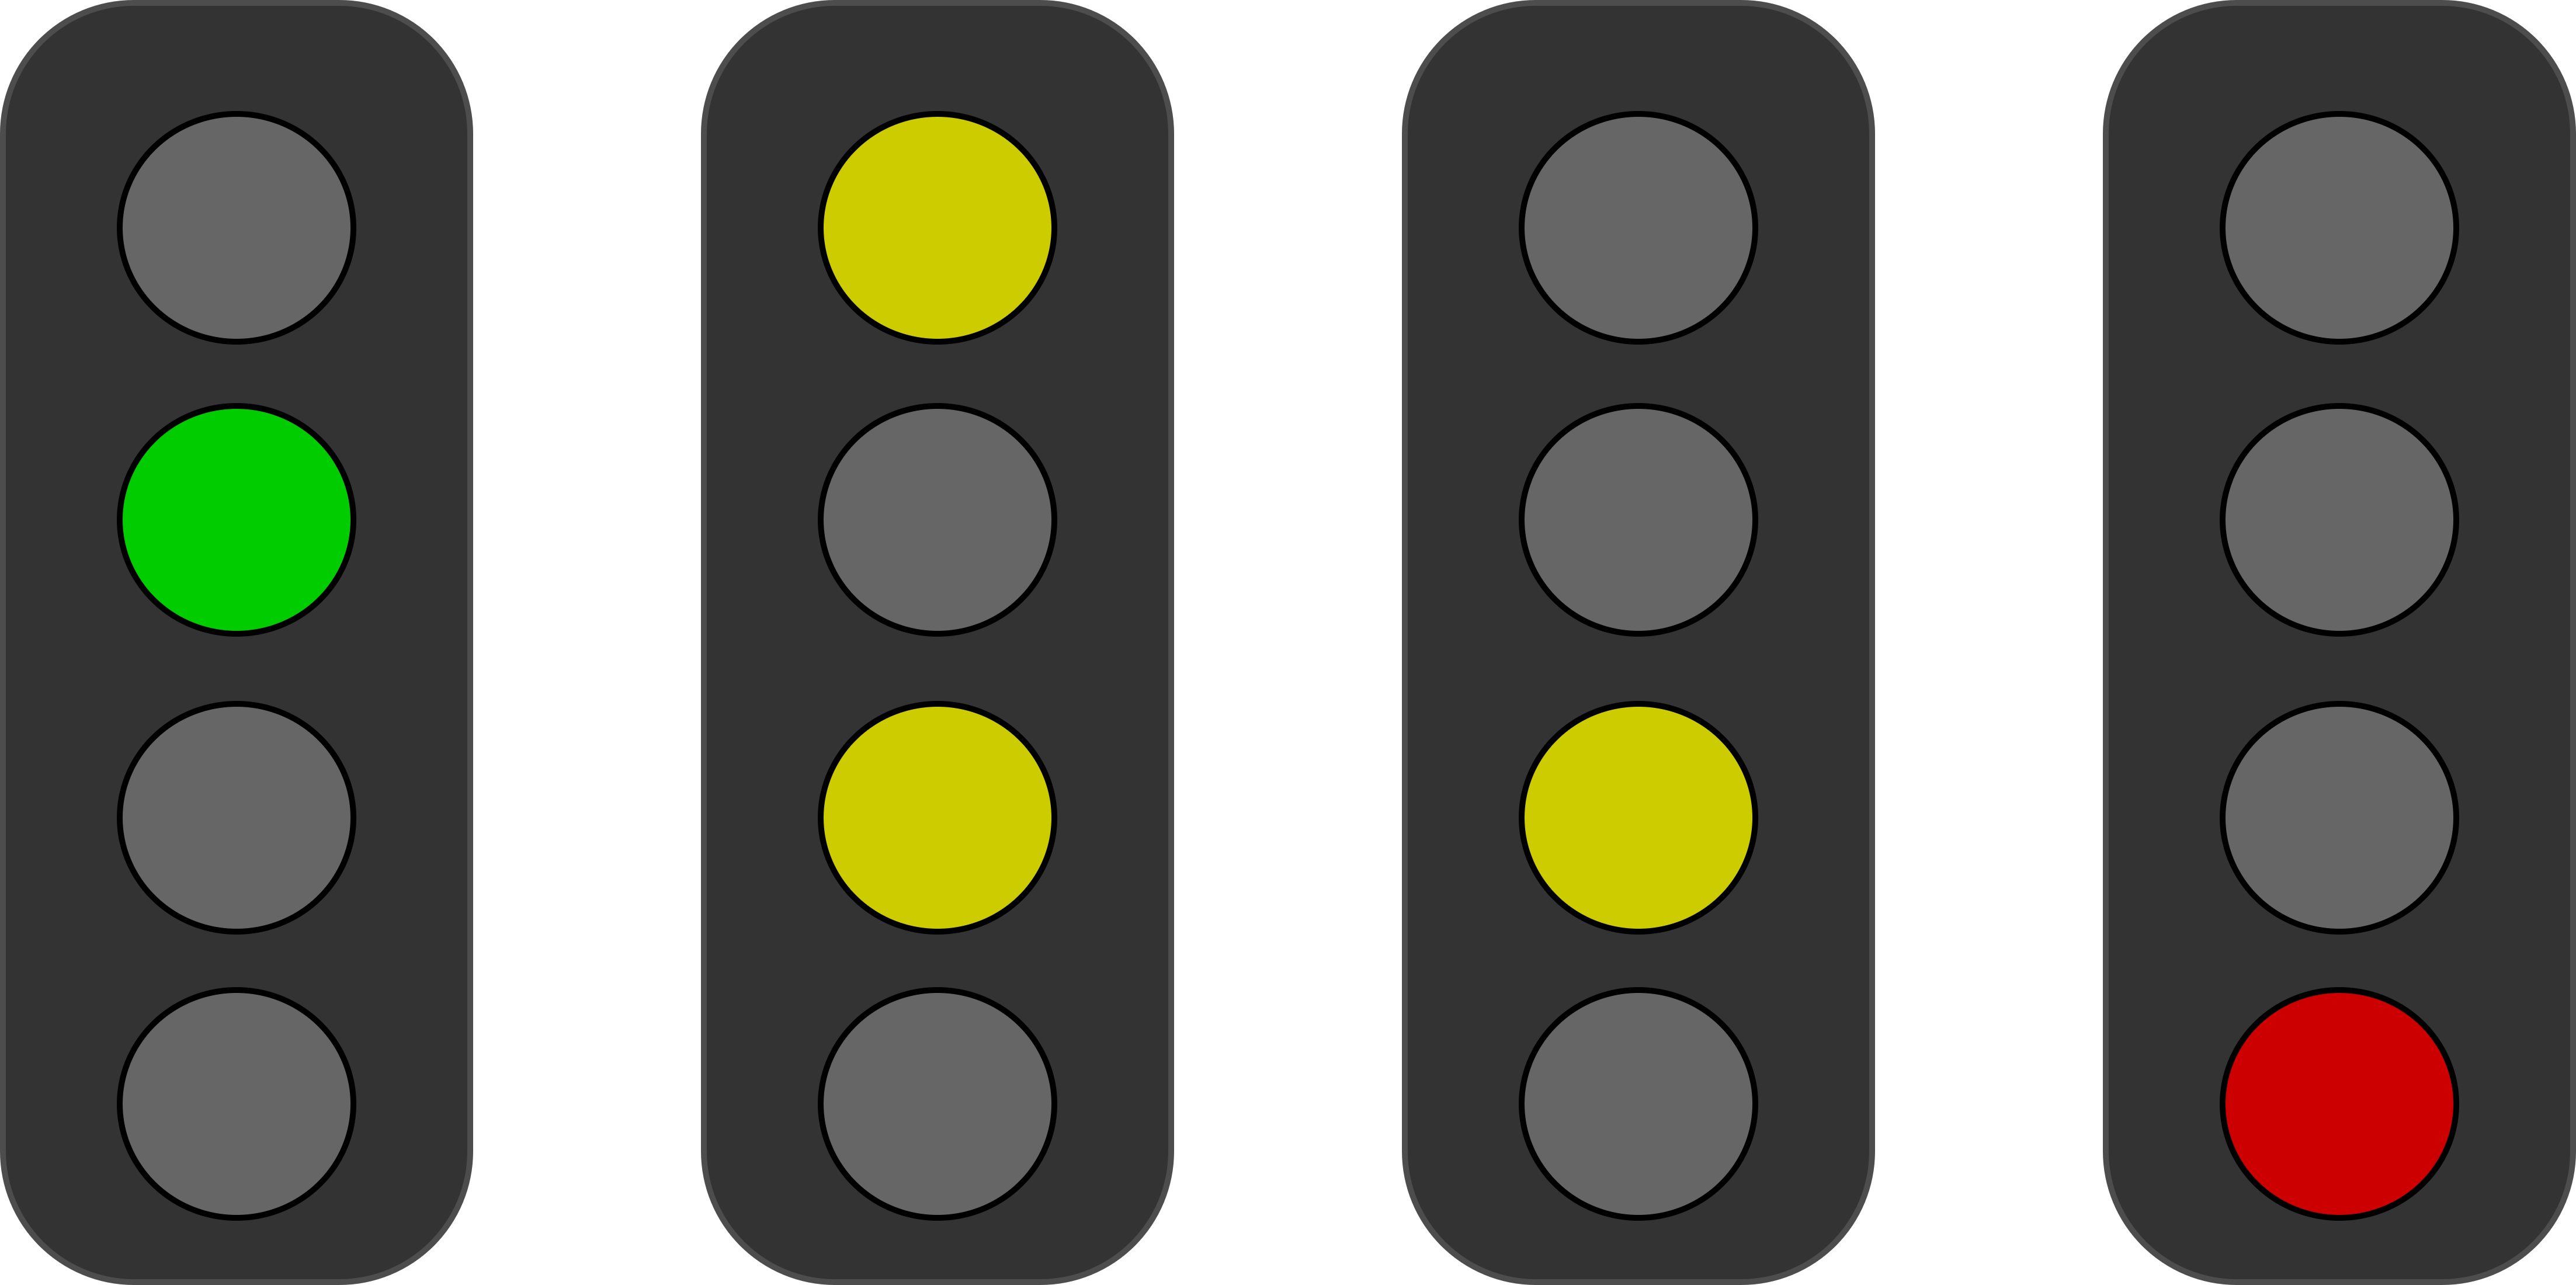
\includegraphics[width=0.5\textwidth]{Figuras/semaforo2}
		\centering\caption{Protección por doble recubrimiento.}
		\label{fig:uk_signalling}
	\end{figure}
	
	En las etapas iniciales del proyecto la única herramienta de visualización era Design4Rail \cite{DESIGN4RAIL}. Esta herramienta solamente puede representar señales de un aspecto y, al no tener todavía implementado el AGG, no era posible representar señales de doble aspecto amarillo. Es por esa razón que el RNA reemplazó la señal doble amarilla por una señal naranja. Este reemplazo también es realizado por el ACG al implementar las señales en VHDL. El proyecto se encontraba en estado muy avanzado cuando se diseñó el AGG, por lo que se mantuvo que todas las señales son de un único aspecto. En este trabajo, por lo tanto, siempre se representará mediante una señal naranja a una señal doble amarilla.
	
	
	%Ya que Design4Rail \cite{DESIGN4RAIL}, el software utilizado para visualizar el señalamiento al inicio del proyecto, solo puede representar señales de un aspecto, en la Figura \ref{fig:ACG_recrubrimiento_1} se reemplazó la señal doble amarilla por una señal naranja. En este trabajo siempre se representará mediante una señal naranja a una señal doble amarilla.

	
	
	\subsection{Liberación secuencial}
	\label{sec:ACG_liberacion}
	
	Esta claro que las rutas conflictivas no pueden ser habilitadas a la vez, pero existen algunas rutas que son parcialmente conflictivas solamente, que comparten una parte de la infraestructura y no toda. La implementación de la liberación secuencial aumenta la flexibilidad en la asignación y habilitación de rutas, mejorando la logística permita por el sistema de enclavamientos. En la Figura \ref{fig:ACG_secuencial_1} se ilustra una formación que iniciará una ruta ya habilitada, para lo cual ya han sido bloqueadas las secciones (coloreadas en naranja) y la infraestructura (coloreadas en rojo).
	
	 \begin{figure}[!h]
	     \centering
	     
\includegraphics[width=1\textwidth]{Figuras/secuencial_1}
	     \centering\caption{Formación iniciando una ruta ferroviaria.}
	     \label{fig:ACG_secuencial_1}
	 \end{figure}
 
	Al ocupar las secciones de vías, debido al bloqueo por ocupación, la señal de inicio de la ruta pasa a peligro y se bloquea la sección consecutiva a la ruta (coloreado en naranja), debido a la protección por solape. Esto se ilustra en la Figura \ref{fig:ACG_secuencial_2}.
	
	\begin{figure}[!h]
    	 \centering
	     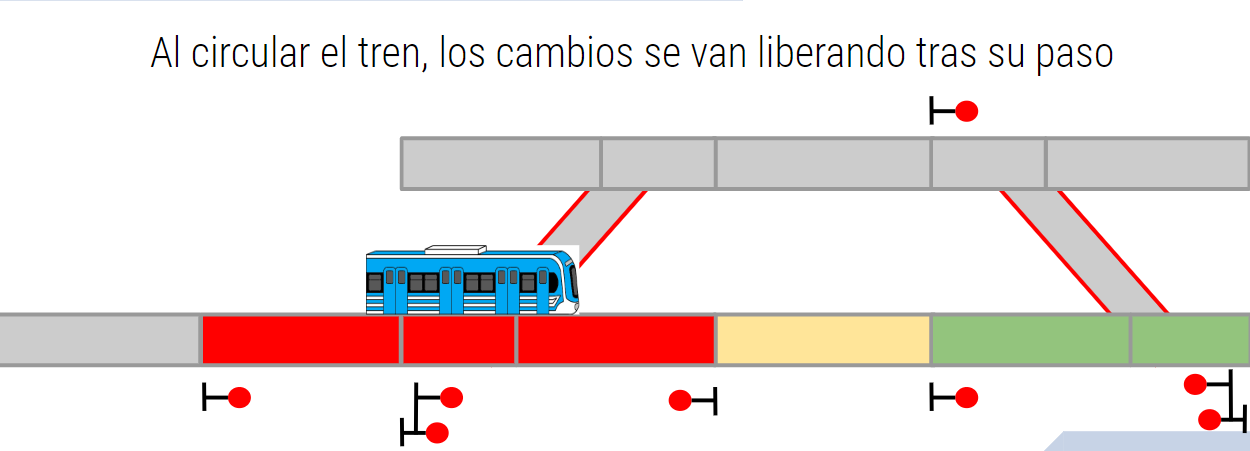
\includegraphics[width=1\textwidth]{Figuras/secuencial_2}
    	 \centering\caption{Formación activando el bloqueo por ocupación y el bloqueo por solape.}
    	 \label{fig:ACG_secuencial_2}
	\end{figure}
 
 	Una vez que la formación desocupa las secciones de vías asociadas al cambio de vías anterior, el sistema de enclavamientos libera inmediatamente toda la infraestructura asociada, como se ilustra en la Figura \ref{fig:ACG_secuencial_3}. A la vez, el sistema de enclavamientos debe esperar a que se cumpla el plazo de seguridad antes de liberar la infraestructura posterior al fin de la ruta. Solamente son liberadas las secciones y señales que ya no son conflictivas.
	   
	\begin{figure}[!h]
	  \centering
	  
\includegraphics[width=1\textwidth]{Figuras/secuencial_3}
	  \centering\caption{Liberación secuencial de la infraestructura por detrás de la formación.}
	  \label{fig:ACG_secuencial_3}
	\end{figure}
 
 	Transcurrido el tiempo de seguridad, el sistema de enclavamientos libera las secciones, cambios de vías, señales y toda infraestructura posterior al fin de la ruta, tal como se ilustra en la Figura \ref{fig:ACG_secuencial_4}.

	 \begin{figure}[!h]
	     \centering
	     
\includegraphics[width=1\textwidth]{Figuras/secuencial_4}
	     \centering\caption{Liberación secuencial de la infraestructura por delante de la formación.}
	     \label{fig:ACG_secuencial_4}
	 \end{figure}
	    
	El ACG implementa estas funcionalidades de seguridad para cada sistema de enclavamientos generado. 
	
	En las siguientes secciones se profundizará en la implementación de cada uno de los módulos del sistema y su comportamiento dinámico.